\documentclass{beamer}
\usetheme[
    sectionpage=progressbar,
    progressbar=foot
]{metropolis}             % Use metropolis theme
\setsansfont[	 	  % Fix needed to make fonts work: https://github.com/matze/mtheme/issues/280
    Extension      = .otf,
    UprightFont    = *-Light,
    ItalicFont     = *-LightItalic,
    BoldFont       = *-Regular,
    BoldItalicFont = *-RegularItalic
]{FiraSans}
\setmonofont[
    Extension   = .otf,
    UprightFont = *-Regular,
    BoldFont    = *-Medium
]{FiraMono}
\usepackage[german]{babel}
\definecolor{cioDarkBlue}{HTML}{12254c}
\setbeamercolor{normal text}{%
    fg=cioDarkBlue,
    bg=black!2
}
\graphicspath{ {img/} }

\title{Was sind Linux Container und wie funktionieren sie?}
\date{\today}
\author{Anian Ziegler}
\institute{cioplenu}
\begin{document}
  \maketitle
  \section{Einführung}
  \begin{frame}{Was sind Container?}
    Hello, Hackerkiste!
  \end{frame}

  \section{Betriebssystem Virtualisierung}
  \begin{frame}{Was sind Container?}
    Hello, Hackerkiste!
  \end{frame}
  \begin{frame}{Was sind Container?}
    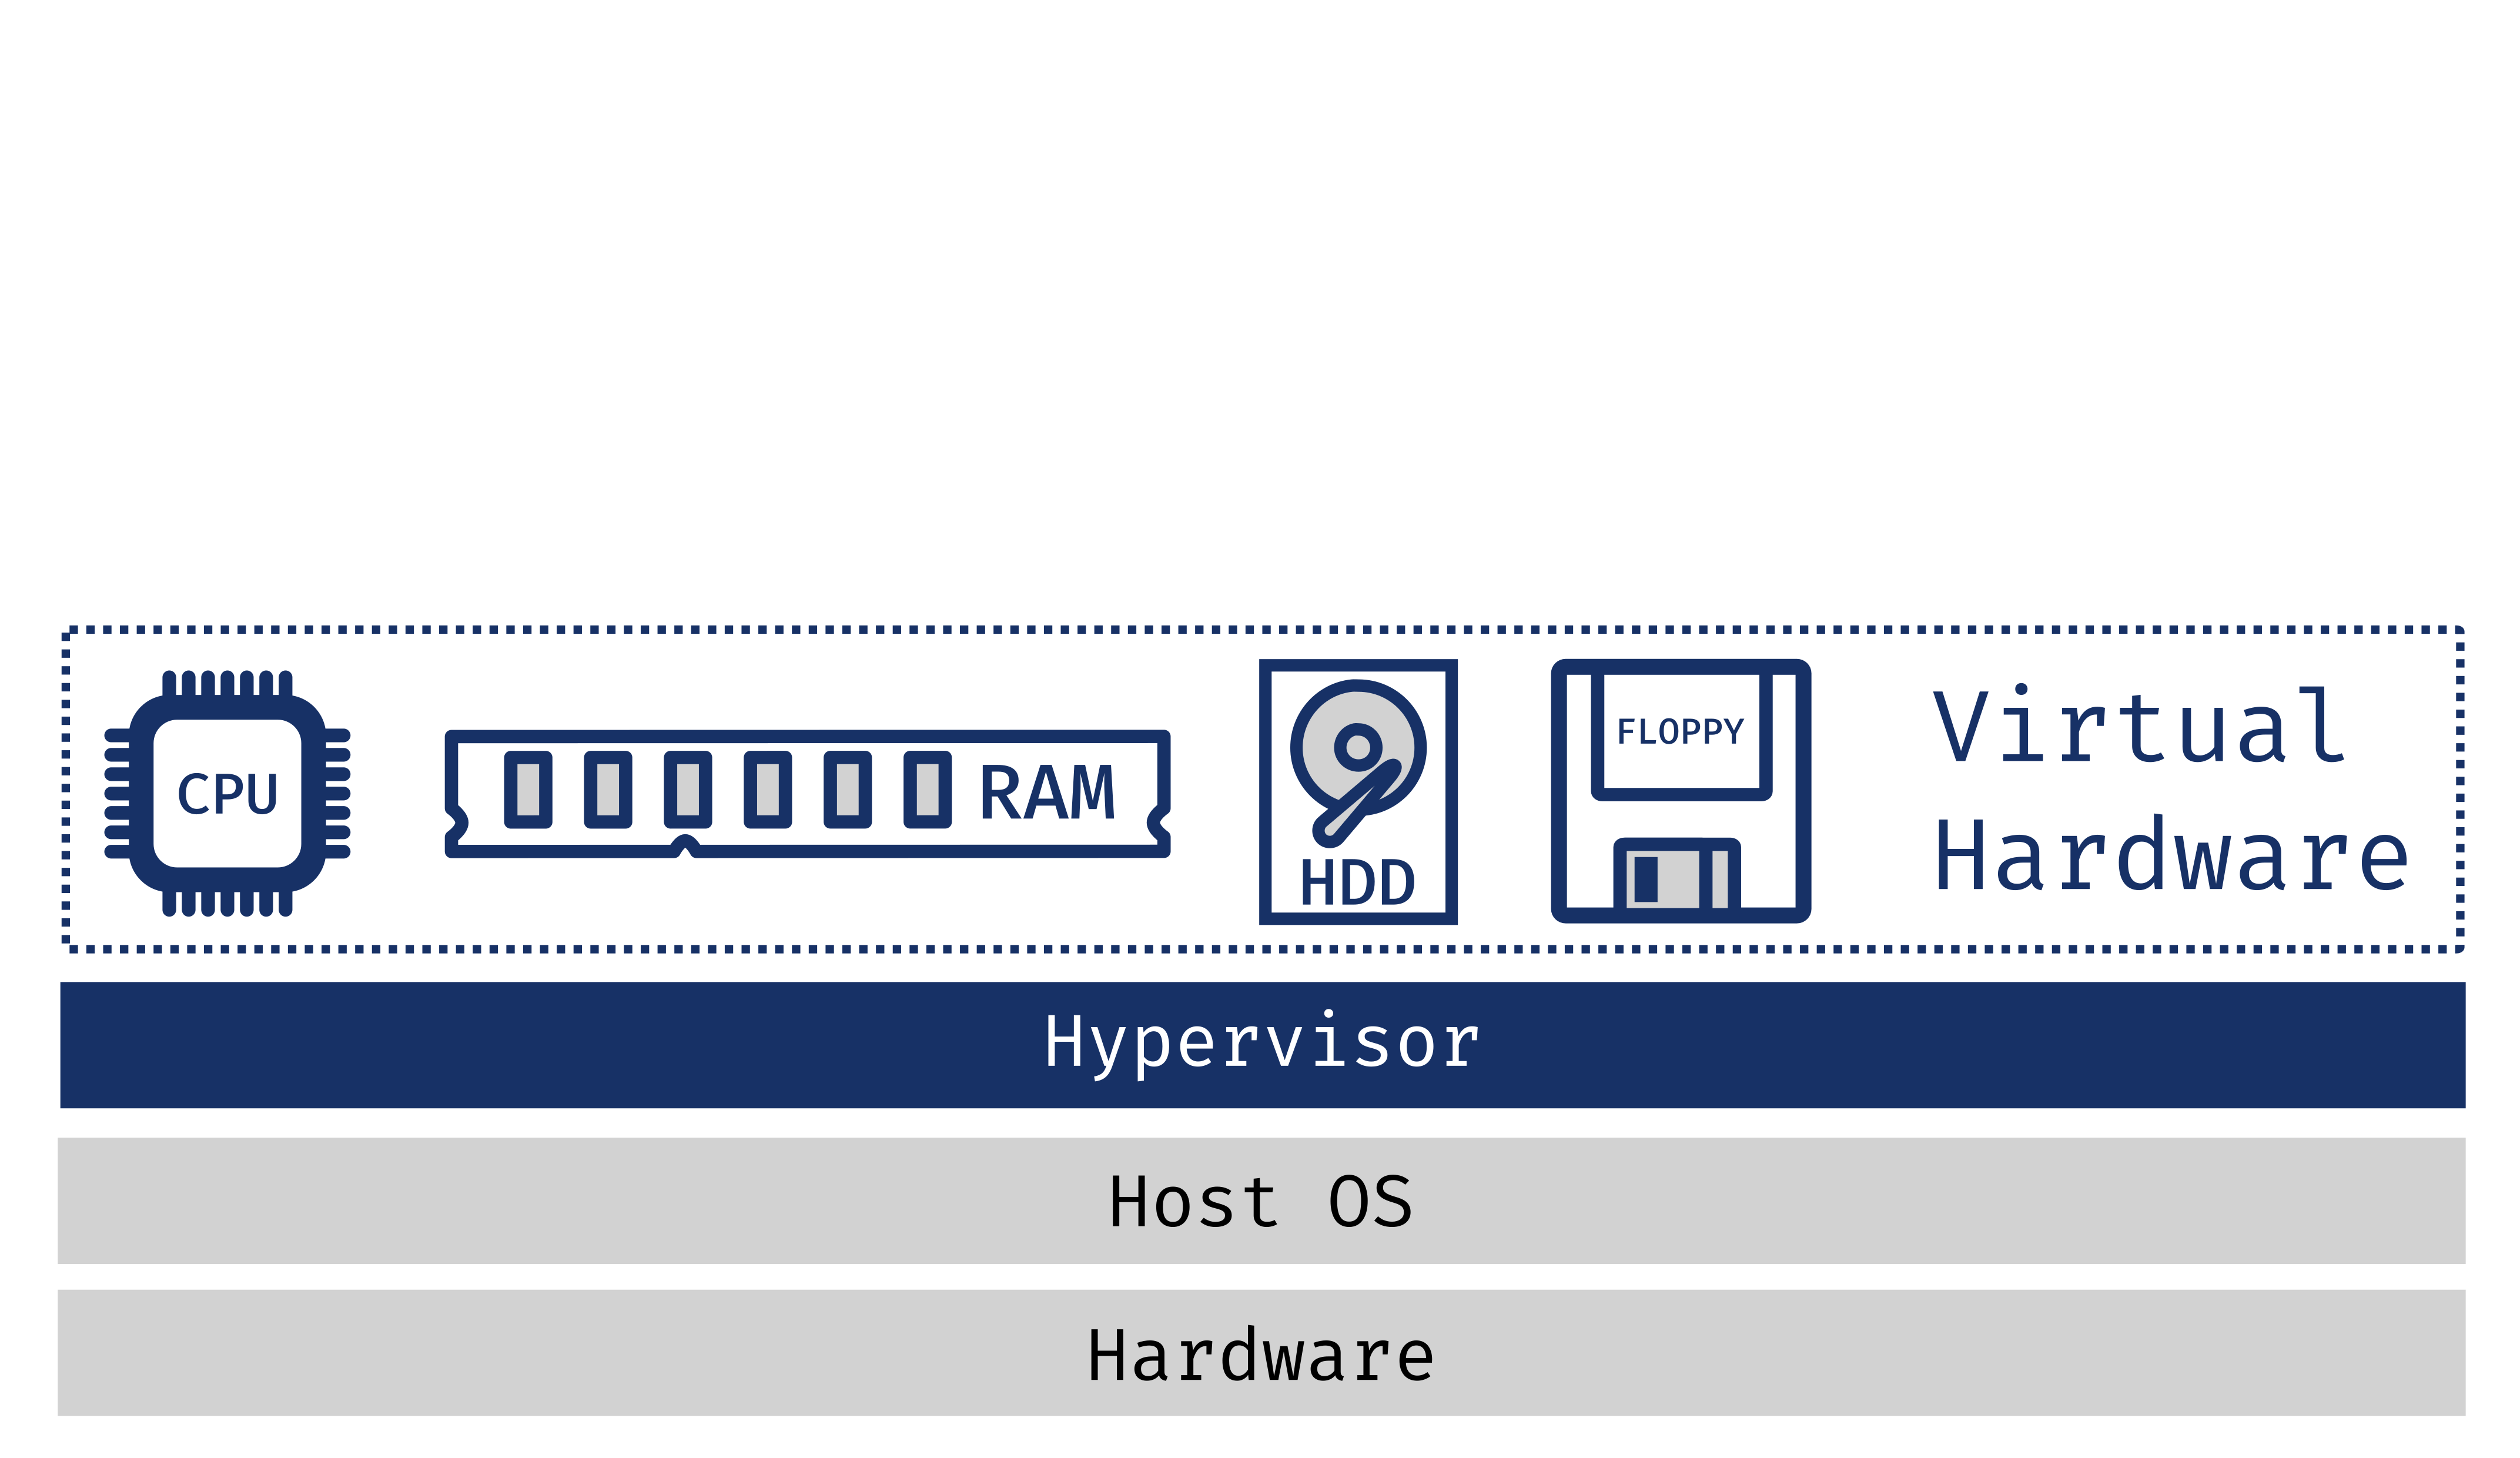
\includegraphics[width=\textwidth]{hypervisor}
  \end{frame}
  \begin{frame}{Was sind Container?}
    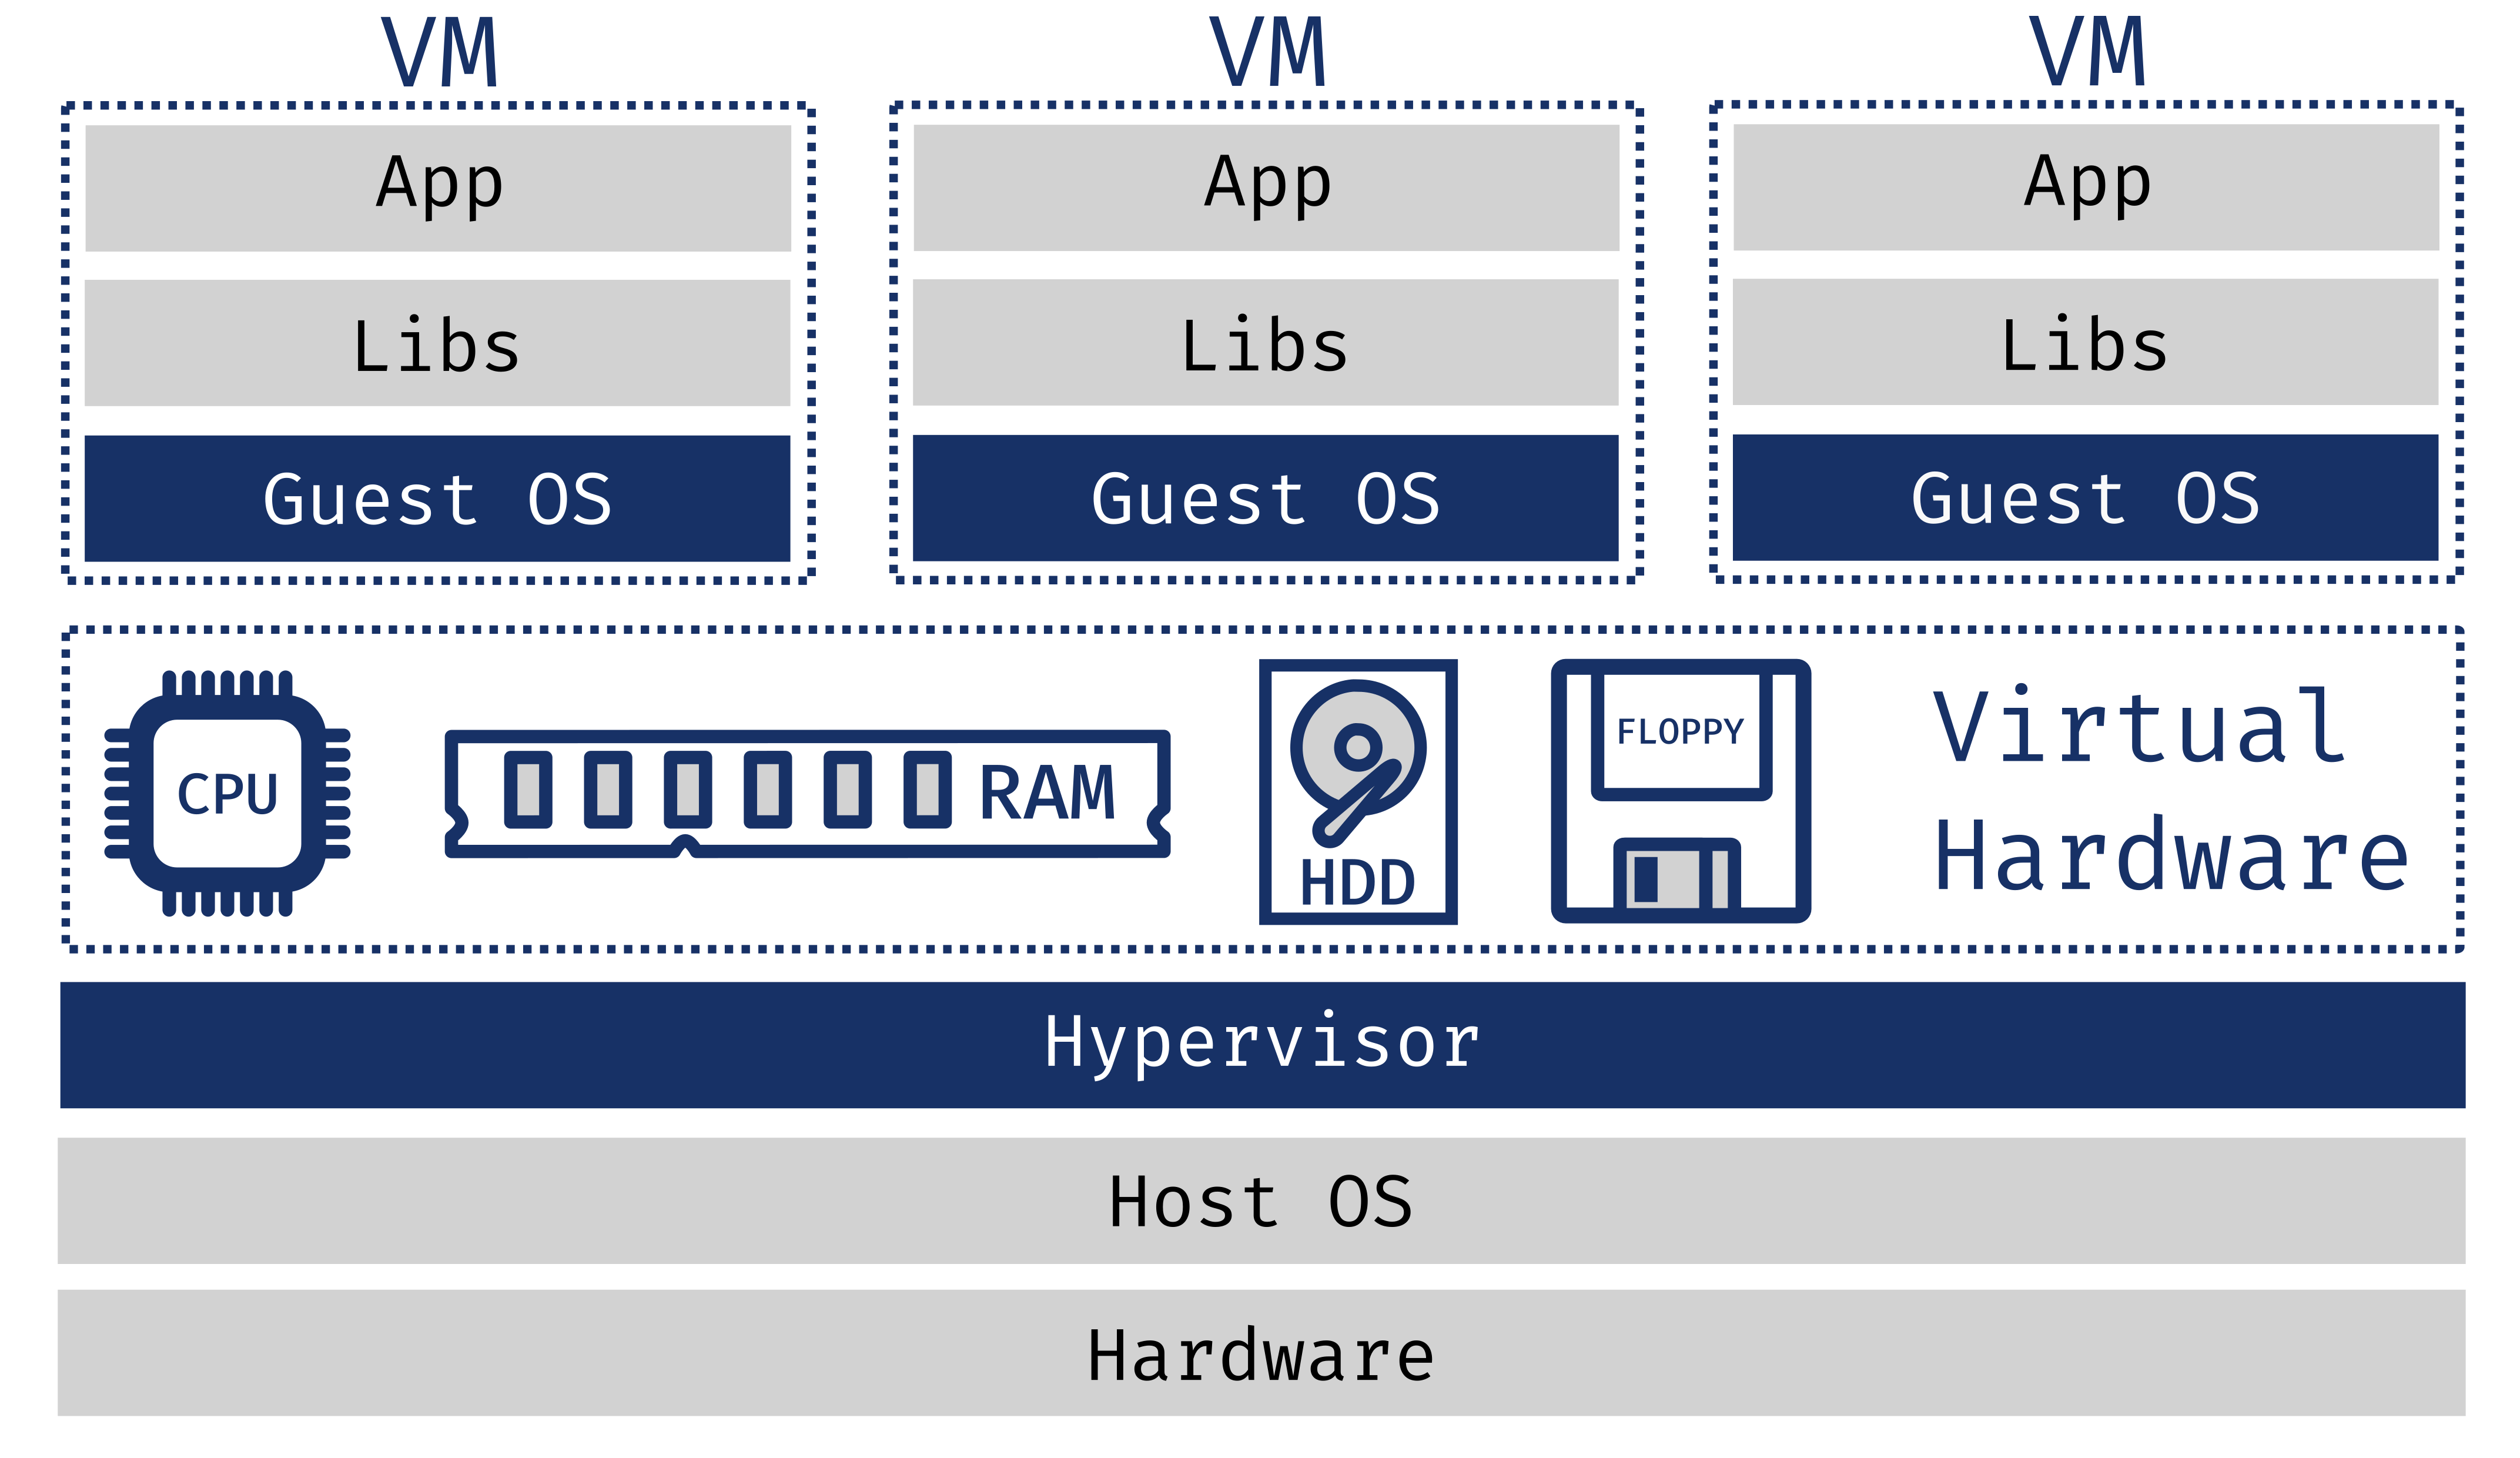
\includegraphics[width=\textwidth]{vms}
  \end{frame}
  \section{Geschichte}
  \begin{frame}{Was sind Container?}
    Hello, Hackerkiste!
  \end{frame}
  \begin{frame}[standout]
    Fragen?
  \end{frame}
\end{document}

